\documentclass[12pt]{article}

\usepackage[betterproportions,european]{circuitikz}
\usepackage{siunitx}

\ctikzset{bipoles/thickness=1}
\tikzset{bookcircuit/.style={line width=1pt,scale=1.25}}

\usepackage{charter}

\begin{document}
hallo

\begin{center}
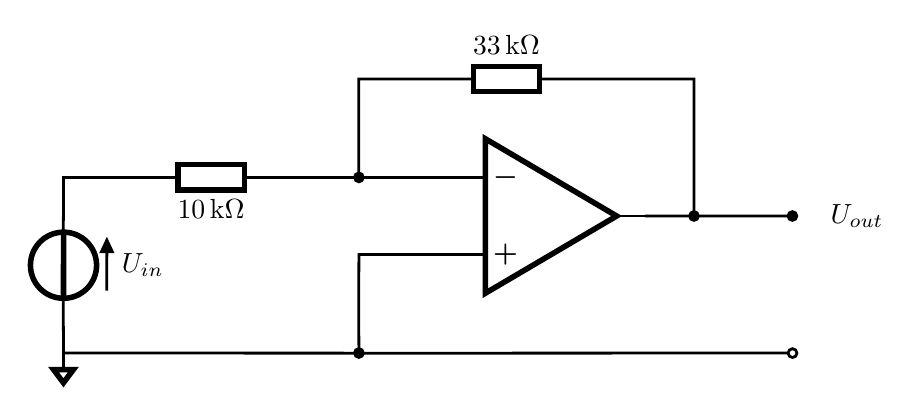
\begin{tikzpicture}[bookcircuit]

\draw (0, 0) node[op amp] (opamp) {}
      (opamp.-) to[short,-*] ++(-1, 0) coordinate (A)
%      (opamp.+) -| ++(-1,-1) coordinate B) %node[sground] (B) {}
      (opamp.+) to [short] ++(-1,0)
      to [short,-*] ++(0,-1) coordinate (B)
      (opamp.out) to [short,-*] ++(.5, 0) coordinate (X)
      to[short, -*] ++(1,0) coordinate (C) node[right,xshift=10pt] {$U_{out}$}
%      to [short] ++(0,0) coordinate (C)
      (C |- B) coordinate (XXX) %node[sground]{}  %node[ocirc]{}
      (A) to[R, l=\SI{10}{\kilo\ohm}] ++(-3, 0) coordinate (D) %-- ++(-1, 0) coordinate (D)
      to [V<=$U_{in}$] (D |- B) coordinate (null) node[sground]{}
      (A) |- ++(0,1) coordinate (L1)
%      to [R=\SI{33}{\kilo\ohm}] ++(2,0) -| (opamp.out)
      to [R=\SI{33}{\kilo\ohm}] ++(3,0) -| (X)
%      to [R=\SI{33}{\kilo\ohm}] ++(2,0) -| (X)
%      to[short,-o] ++(1,0)
%     to [short] {0,0}
(null) to [short,-o] (XXX)
%       () [R] (XXX)
;

\end{tikzpicture}
\end{center}

\end{document}